\documentclass{standalone}
\usepackage{tikz}
\usepackage{ctex,siunitx}
\setCJKmainfont{Noto Serif CJK SC}
\usepackage{tkz-euclide}
\usepackage{amsmath}
\usetikzlibrary{patterns, calc}
\usetikzlibrary {decorations.pathmorphing, decorations.pathreplacing, decorations.shapes,}
\begin{document}
\small
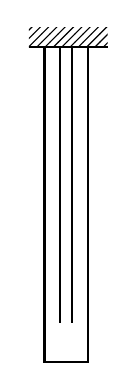
\begin{tikzpicture}[>=stealth, thick]
  % \useasboundingbox(-1,-0.75)rectangle(3.7,1.4);
  \fill [pattern = north east lines] (0,0) rectangle (1,.25);
  \draw(0,0)--(1,0);
  \draw (.2,-4) rectangle (.75,0);
  \draw(.4,0)--(.4,-3.5);
  \draw(.55,0)--(.55,-3.5);
  \end{tikzpicture}
\end{document}